% GitHub's web editor with its own search bar open.
% The instructor's capture from week 4 (slides/week-04/img/handout_editor_search.png), with
% numbered markers. Build with `make figures` in handouts/, which writes
% editor-search_annotated.pdf and editor-search_annotated.png. Coordinates are pixels of
% the 700 x 345 capture.
\documentclass[border=0pt]{standalone}
\makeatletter\def\input@path{{../../common/}{handouts/common/}}\makeatother
\usepackage[scaled=0.92]{helvet}
\usepackage{graphicx}
\usepackage{handoutmarkers}
\begin{document}
\setlength{\unitlength}{0.0064286in}% 1 px of the 700-px capture; the figure is 4.5in wide
\begin{tikzpicture}[x=\unitlength,y=-\unitlength,
    every node/.append style={draw=white,line width=0.7pt}]
  \node[anchor=north west,inner sep=0,draw=none] at (0,0)
    {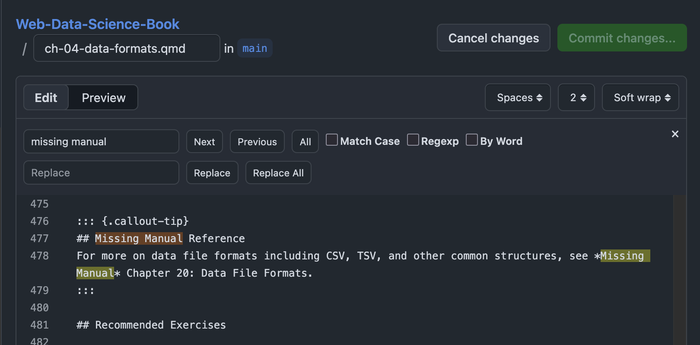
\includegraphics[width=700\unitlength]{../../../slides/week-04/img/handout_editor_search.png}};
  \draw[black!25] (0,0) rectangle (700,345);
  \node[marker] at (158,141) {1};                 % the editor's search box
  \node[marker] at (268,238) {2};                 % the line it found
\end{tikzpicture}
\end{document}
